\section*{Problem 3}

The task is to implement John Horton Conway's Game of Life.

The solution is structured as a front-end class \code{GameOfLifeMain} which
handles input and output and a backend class \code{GameOfLife} which handles
the game logic.

When \code{GameOfLife} is instantiated, the \emph{world} is setup. The world
is represented as a two dimensional array of integers. This two dimesional
array can also be provided, in such a case all rows must be the same length as
the number of columns -- it must be a square.

On this instance of the class (the Game of Life World) the method
\code{nextState} calculates the next state of all cells in the world. To do
this the method \code{liveNeighbours} is used. \code{LiveNeighbours}
calculates the number of live neighbouring cells to a point in the world. The
method accounts for over- and underflowing the coordinate system. If a
neighbour is past the right edge of the world, the coordinate is instead set
the neighbour on the left edge. This gives the world the topology of a torus.

Random noise can be introduced to world using the method \code{cosmicNoise}.
The method takes an argument $p$ which is the probability a cell has toggling
state. 
\begin{figure}
        \centering
        \begin{subfigure}[b]{0.3\textwidth}
				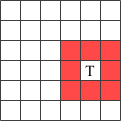
\includegraphics{Normal-target}
                \caption*{A normal target}
        \end{subfigure}%
        ~
        \begin{subfigure}[b]{0.3\textwidth}
				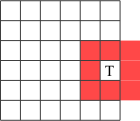
\includegraphics{Off-target}
                \caption*{A targer with overlapping}
        \end{subfigure}
         ~
        \begin{subfigure}[b]{0.3\textwidth}
				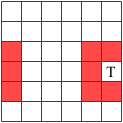
\includegraphics{Off-target-adjusted}
                \caption*{Adjusted neighbour cells}
        \end{subfigure}
\end{figure}

Running the program

\begin{Verbatim}
java GameOfLife
\end{Verbatim}

With file input

\begin{Verbatim}
java GameOfLife glider_gun.gol
\end{Verbatim}

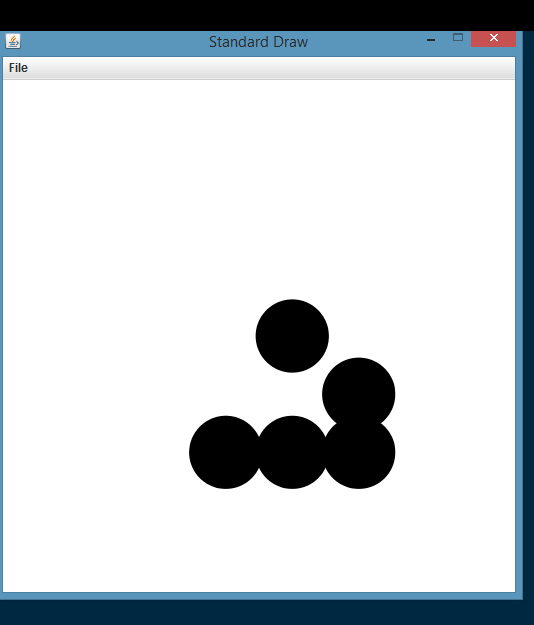
\includegraphics[width=0.5\textwidth]{gol-example}